\section{Quadcopter flight tests}

Once the performance and safety of the control algorithms have been validated in the simulated environment, it is possible to begin flight tests and take to the air with a physical drone.
In this final section of the validation process, all the previous parts are put together to test how the developed software will perform in a real quadcopter during flight.
To do this, first, it will be necessary to build the base vehicle from its development kit and then integrate all the additional pieces needed for this project, like the companion computer and the camera.
Then, after ensuring the vehicle can fly with all the payload through remote control, both of the developed solutions will be tested.
First, the hand-control solution to verify that the autopilot can receive flight commands from an offboard computer and second, the follow solution to confirm that the companion computer can function as well during flight with its dedicated power supply as it did when it was stationary.

The exact steps that will be executed one after the other to ensure that safety is maintained during the whole process are as follows:

\begin{enumerate}
    \item Build the quadcopter with its basic components.
    \item Add custom payload.
    \item Fly with remote control and factory autopilot only, monitoring through QGroundControl.
    \item Fly with custom software from offboard computer with \texttt{test-camera} tool (\ref{subsec:cam-tool}).
    \item Fly with \texttt{test-camera} tool from onboard computer.
    \item Fly with custom hand-gesture control solution from offboard computer.
    \item Fly with custom follow solution from onboard computer.
\end{enumerate}

\subsection{Build process}
\label{sec:test-7-builddrone}

% Setup:    build drone, configuration, calibration
% Test:     - RC, GPS, 
%           - Arm, takeoff commands
%           - Camera holder
% Results:  wiring, drone pictures, QGroundControl calibration screens
%           holder 3d, drone close-up, camera feed


As mentioned before, the vehicle used in this project is the Holybro X500, a drone designed to work with PX4.
The detailed instructions to build the vehicle from its Development Kit can be found in the PX4 documentation \footnote{\url{https://docs.px4.io/main/en/frames_multicopter/holybro_x500_pixhawk4.html}}.
Figure \ref{fig:x500-dev-kit} shows all the parts that make up the complete vehicle.

\begin{figure}
  \centering
  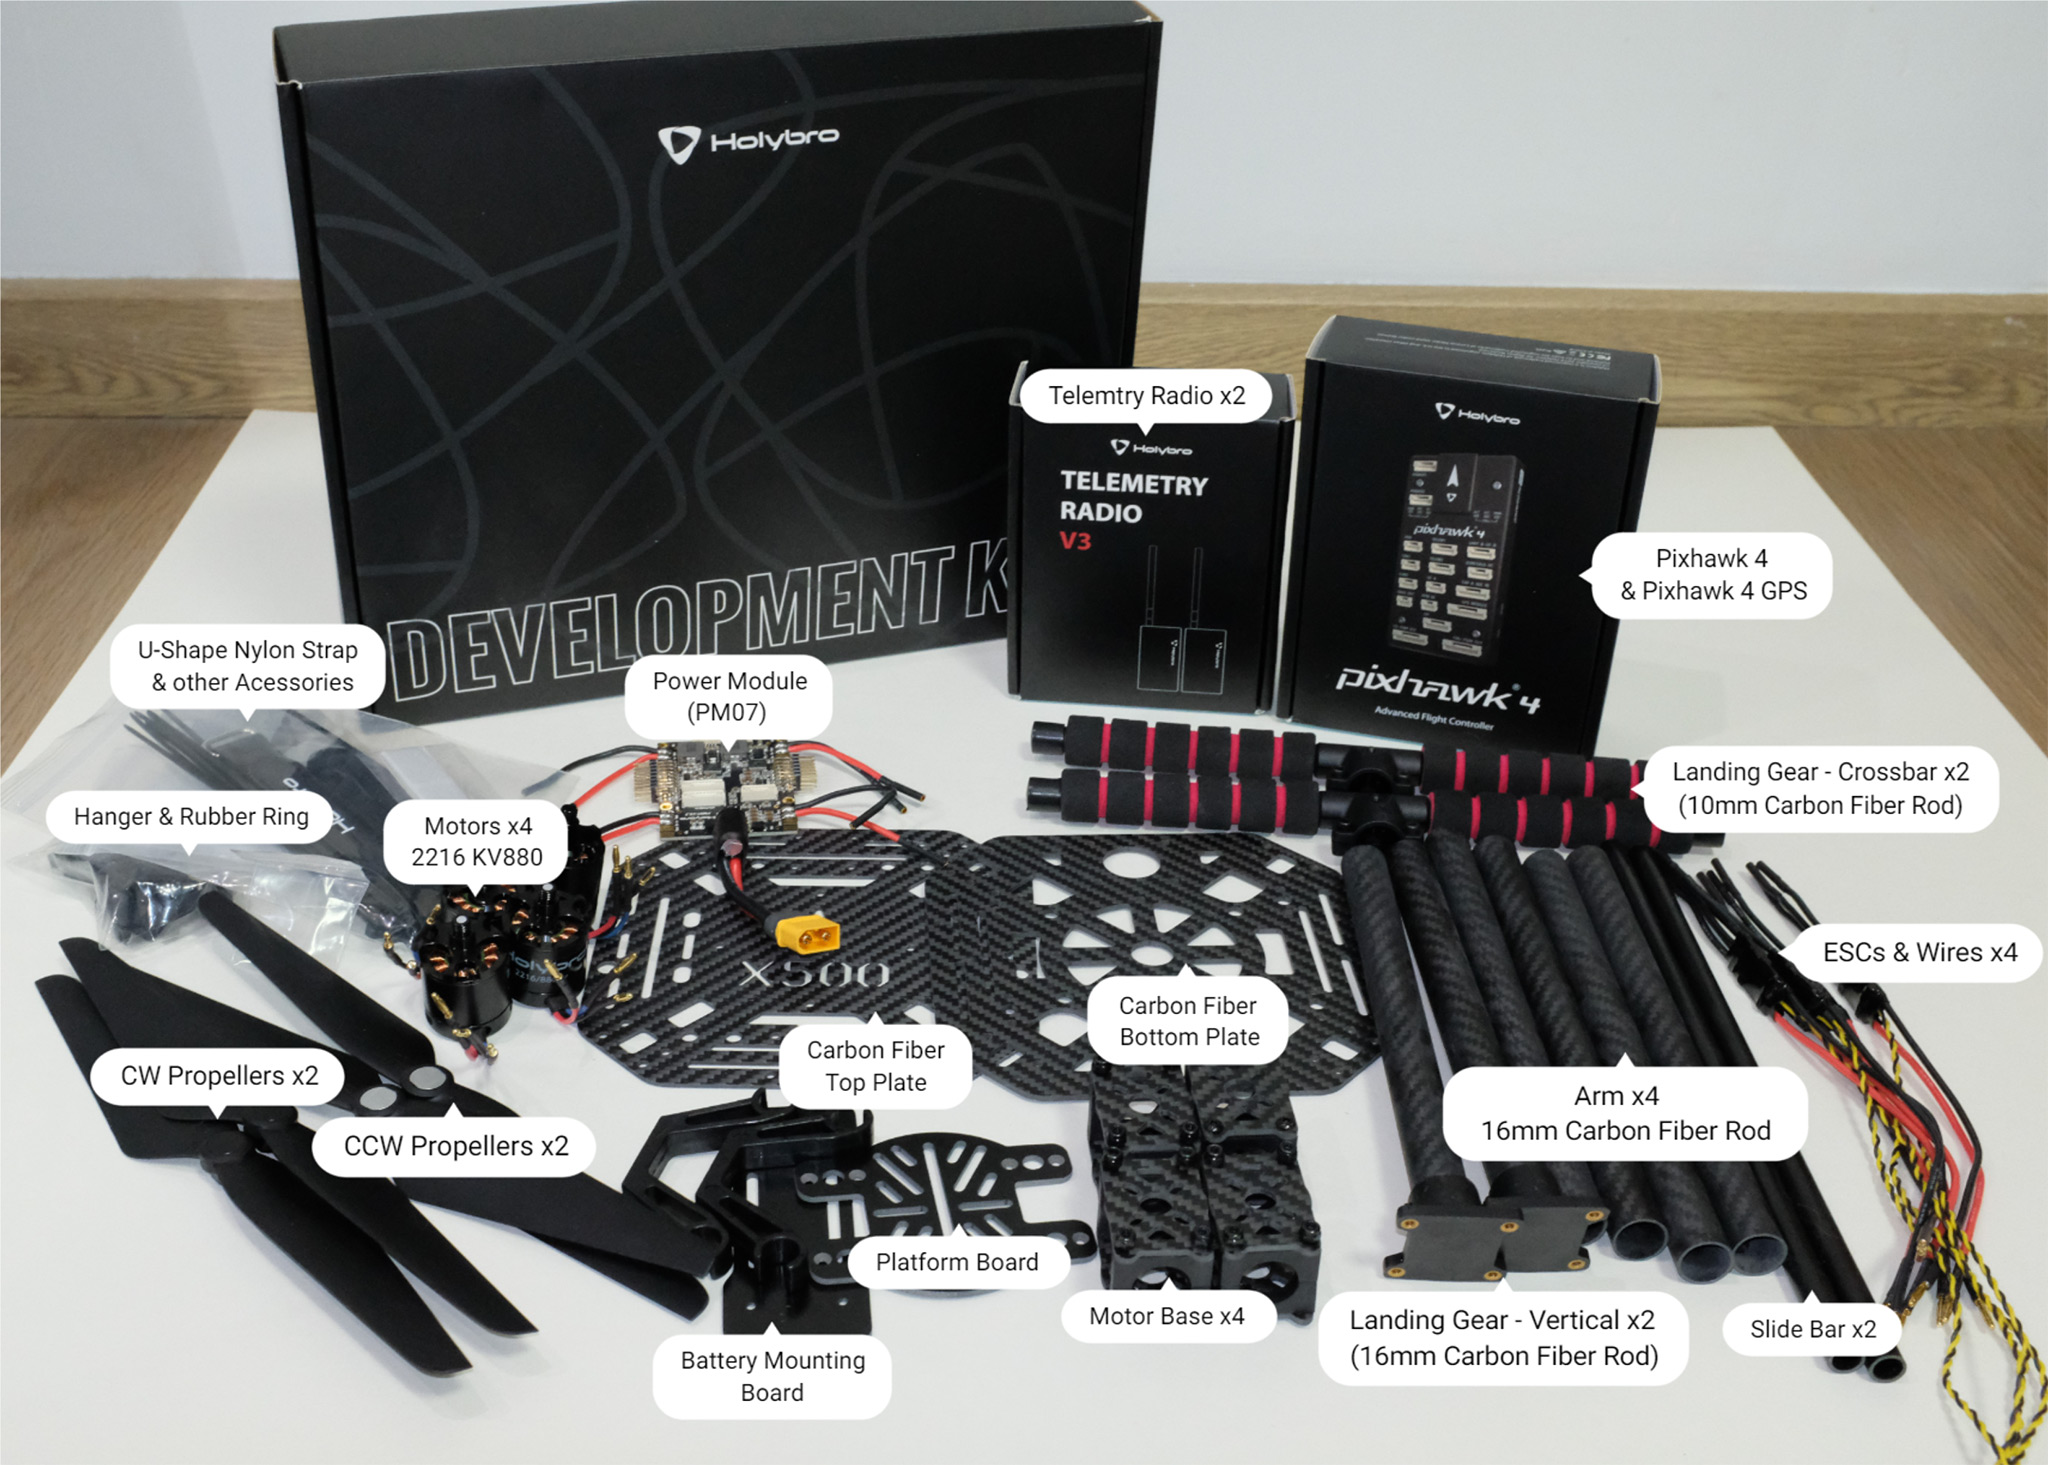
\includegraphics[width=.6\textwidth, keepaspectratio]{img/x500-dev-kit.jpg}
  \caption{Development kit for the Holybro X500.}
  \source{Adapted from \citetitle{px4-guide} \cite{px4-guide}.}
  \label{fig:x500-dev-kit}
\end{figure}


After all the standard parts are assembled, the custom additions can also be attached using the remaining space in the frame.
The Raspberry Pi companion computer will sit just behind the autopilot to counterbalance the more weighted front of the vehicle where the GPS antenna is located.
This location also allows an easy connection between the autopilot and Raspberry's I/O pins with short cables so as not to clutter the frame with wires excessively.

While in flight, the Raspberry Pi will be powered through a dedicated external battery that outputs power through a 2-ampere USB port.
This port will be connected with the Raspberry Pi's original power cable to its USB-C power supply socket.
As detailed in \ref{sec:test-5-rpi}, this current is enough to power the connected camera and run the developed software with acceptable performance.
This battery will be located underneath the autopilot, centred in the vehicle's frame, so its weight destabilizes it as little as possible, as shown in figure \ref{fig:full-build}.

The camera also needs to be securely attached to the vehicle's frame, with the custom support described in section \ref{subsec:onboard}.
The holder attaches to the slide bars underneath the vehicle's main frame so that the camera and its substantial weight are situated as close to the centre of mass as possible behind the GPS platform.
The battery powering the engines and the autopilot, which is located on the underside of the carbon frame, is also moved slightly backwards from its centred position to make space for the camera and compensate for its weight in the front.
Figure \ref{fig:camera-holder-closeup} shows how the vehicle's underside looks with the camera attached.

\begin{figure}
  \centering
  
\includegraphics[width=0.8\textwidth, keepaspectratio]{img/placeholder.png}
  \caption{Complete build of the quadcopter with the main components highlighted}\label{fig:full-build}
\end{figure}
\todo[inline]{Figure \ref{fig:full-build}: take picture of complete build and annotate with arrows}

\begin{figure}
  \centering
  
\includegraphics[width=0.8\textwidth, keepaspectratio]{img/placeholder.png}
  \caption{Underside of the vehicle, with supports holding the main battery and the camera in place}
  \label{fig:camera-holder-closeup}
\end{figure}
\todo[inline]{Figure \ref{fig:camera-holder-closeup}: take picture of underside showing battery and camera holder}


After the vehicle has been built, there are additional installation and calibration steps that must be carried out before it can fly, also contained in the guide mentioned above.
Any simulation modes previously activated for testing must be deactivated from the Safety section of the vehicle configuration and the \texttt{MAV\_1\_CONFIG} parameter set to \texttt{TELEM2}, as described in section \ref{subsec:offboard}.
Then all the different sensors present, both embedded on the flight controller board and attached to the outside frame, need to be calibrated for this particular build.
The QGroundControl \ref{subsec:qgc} ground station application contains a configuration screen with all the calibration tools needed for the vehicle setup, shown in figure \ref{fig:qgc-config}.
The vehicle can be configured either by connecting the flight controller directly to the computer via the micro-USB port on its side or through a wireless connection by plugging the companion telemetry radio into the computer running QGroundControl.


\begin{figure}
  \centering
  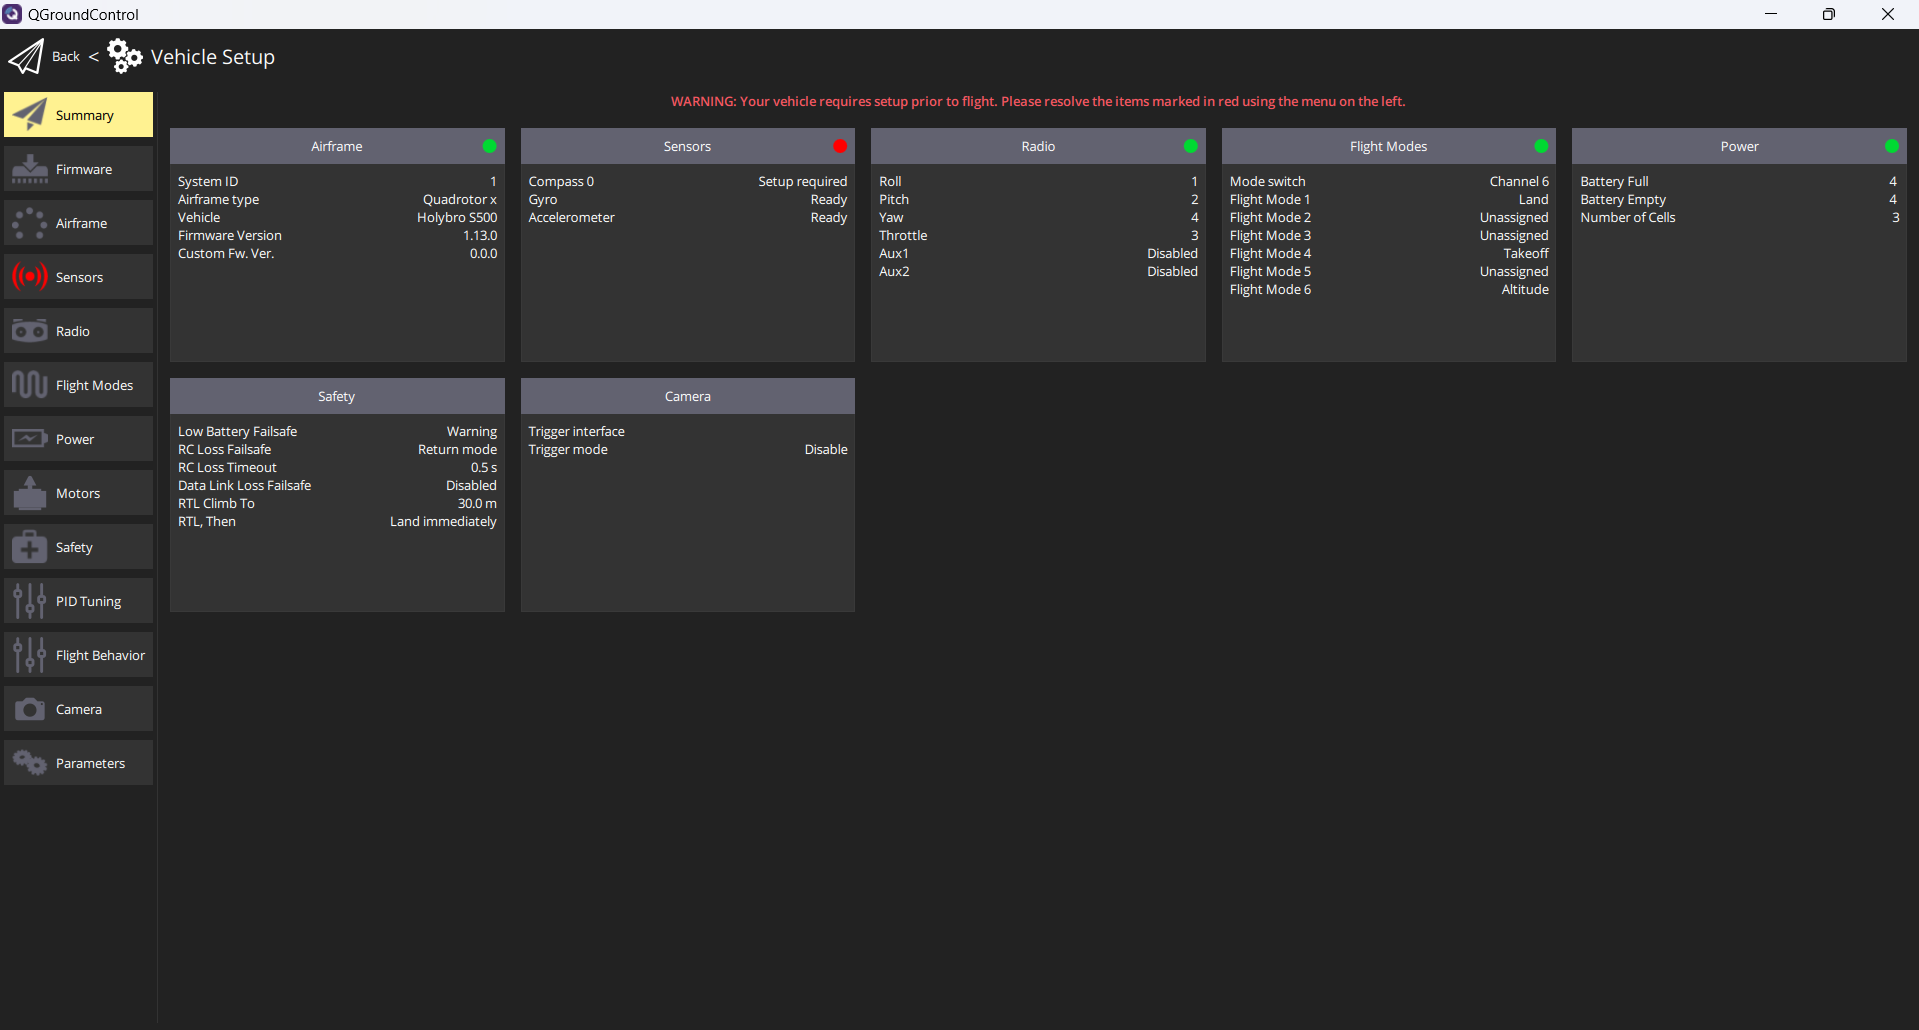
\includegraphics[width=0.45\textwidth, keepaspectratio]{img/qgc-config-1.png}
  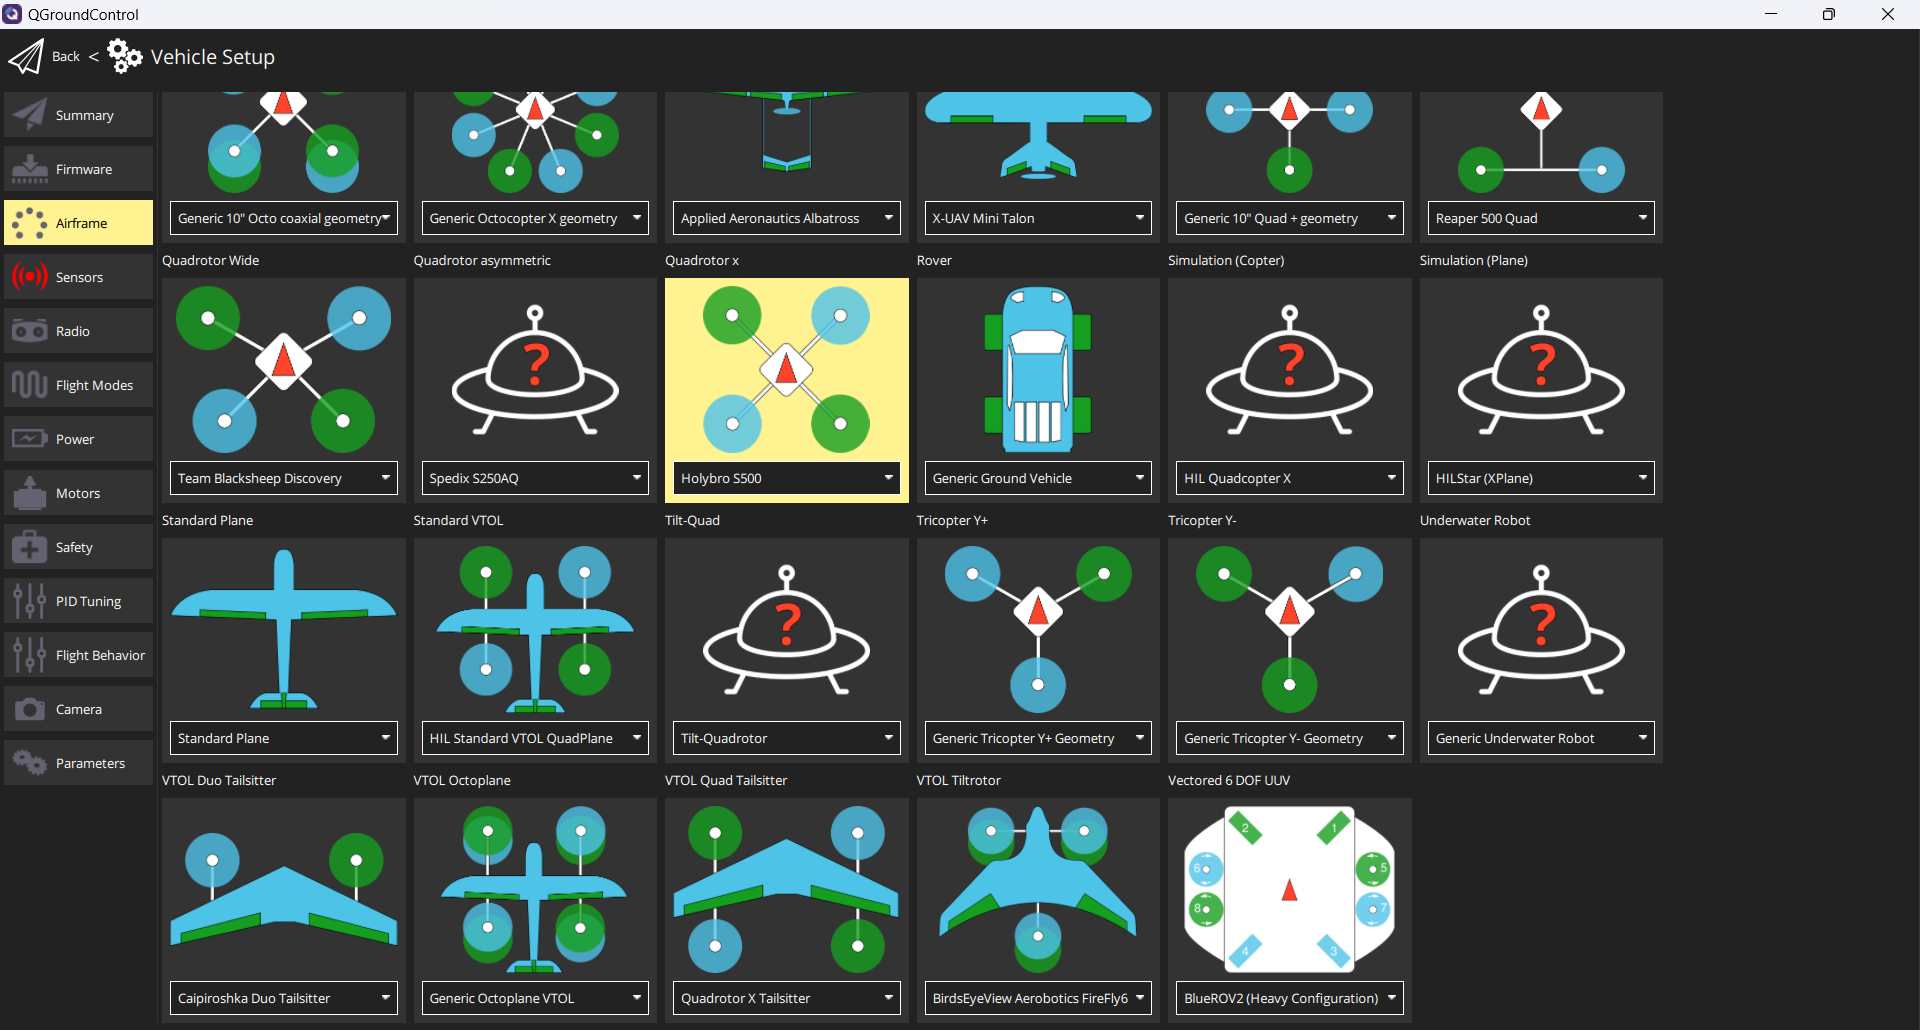
\includegraphics[width=0.45\textwidth, keepaspectratio]{img/qgc-config-3.png}\\
  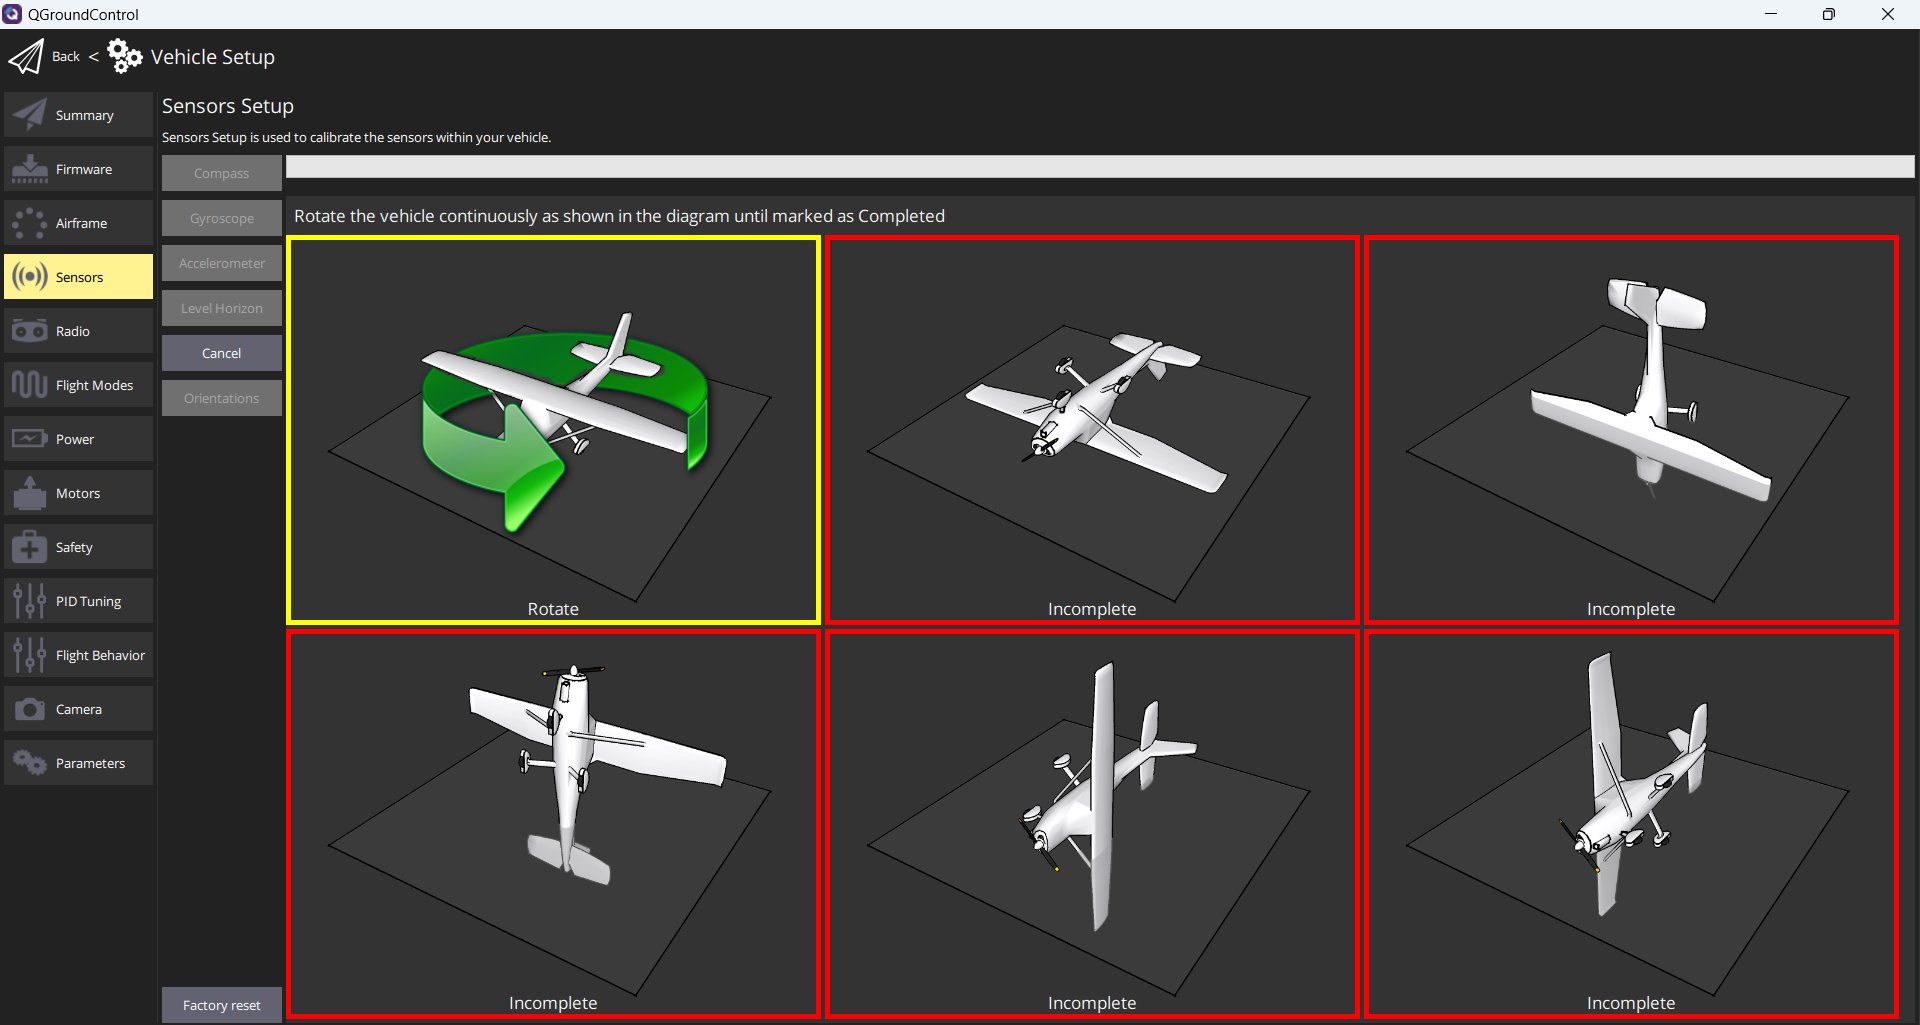
\includegraphics[width=0.45\textwidth, keepaspectratio]{img/qgc-config-2.png}
  \caption{Screenshot from the QGroundControl calibration and setup tools used to configure the vehicle}\label{fig:qgc-config}
\end{figure}


\subsection{Initial tests}
\label{sec:test-8-flight}

% Setup:    flight plan
% Test:     - assisted takeoff, fly with RC
%           - tools/test_camera + record video
% Results:  video of flying, adjust pid set-point

\subsubsection{Baseline flight with factory software}
\label{subsec:fl-test-1}

Once the vehicle is fully configured, the RC controller and QGroundControl can be used to test assisted takeoff and landing.
At this point, the drone should be able to maintain stable flight while using autopilot-assisted flight modes like Position Mode, where the roll and pitch sticks control the acceleration over the ground of the vehicle in the forward/backward and left/right directions relative to the heading the vehicle is facing.
The throttle controls the speed of ascent and descent. 
With the sticks centred, the vehicle will actively remain locked to a position in 3D space, compensating for wind and other forces.
This is the safest manual mode to test that the standard autopilot works as expected.

Through QGroundControl it is possible to map the different switches in the RC controller to various autopilot commands.
For this test, one of the switches with two positions will be mapped to arm/disarm, which controls whether the engines of the quadcopter can start or not. One of the switches with three positions will be mapped to the landing/takeoff/position flight modes, respectively. The main autopilot modes can be tested by switching between the available positions during flight.
This configuration exhausts all the channels available in the RC controller employed.
Other flight modes can be set by using the QGroundControl interface directly.

To carry out the flight, first, the main battery is connected to the socket in the power module.
This starts up the autopilot, the GPS antenna, the telemetry radio, and the RC receiver.
Afterwards, QGroundControl can be started on a computer connected to the second telemetry radio via USB.
If everything has worked correctly, the ground station application will automatically connect to the vehicle and situate its position on a satellite map.
Turning on the RC controller will likewise make it connect to the vehicle, as long as it has been paired correctly, as indicated in the guide linked in the first step of the build process.
Once all the wireless connections have been established, the drone can take off by first switching to the armed state and then switching to the takeoff flight mode.
While the drone is in the air, switching to the position flight mode will allow direct control through the joysticks in the controller.


\subsubsection{Offboard computer flight with test tool}
\label{subsec:fl-test-2}

The second test flight will aim to ensure that the custom software can send takeoff and landing commands through a wireless MAVlink channel from the offboard computer (using the telemetry radio through the developed test tool).
For this flight, the QGroundControl application cannot be connected to the vehicle since the Dronecontrol application will block the telemetry radio channel.
The RC controller will therefore be used as a backup in case anything goes wrong with the software.
At any moment, the controller can switch flight mode and override the input generated from the Dronecontrol application, recovering manual control.
Since the Dronecontrol application can now easily arm the vehicle on its own while sending a takeoff command,
the two-way switch of the controller will be mapped for all the tests from now on to the command to kill the power to the engines.
This command could be helpful in edge cases to protect the vehicle or the surrounding area if the autopilot were to destabilize during takeoff and landing or completely lose control over the vehicle.
Now, once the main battery is connected again to the power module, the test tool is run with the following command for a Windows or a Linux machine, respectively:
\begin{minted}[breaklines, fontsize=\footnotesize, baselinestretch=1]{bash}
dronecontrol tools test-camera -r COM<X>:57600
\end{minted}
or
\begin{minted}[breaklines, fontsize=\footnotesize, baselinestretch=1]{bash}
dronecontrol tools test-camera -r /dev/ttyUSB0:57600
\end{minted}

After successfully connecting to the vehicle, the T and L keys in the computer keyboard can be used for takeoff and landing, respectively. The O key can be used to set the autopilot in offboard flight mode to enable it to receive velocity commands.
Afterwards, the WASD keys can be used to control the forward and sideways velocity of the vehicle and the QE keys to control its yaw velocity.
Figure \ref{fig:flight-test-cam-offboard} displays the output on the computer's terminal window, where the connection process and the sent velocity commands are shown, and the output on the camera from the offboard computer.
A video of the entire process can be found \href{https://l-gonz.github.io/tfg-giaa-dronecontrol/videos/flight-test-offboard}{here}\footnote{\url{https://l-gonz.github.io/tfg-giaa-dronecontrol/videos/flight-test-offboard}}.

\begin{figure}
  \centering
  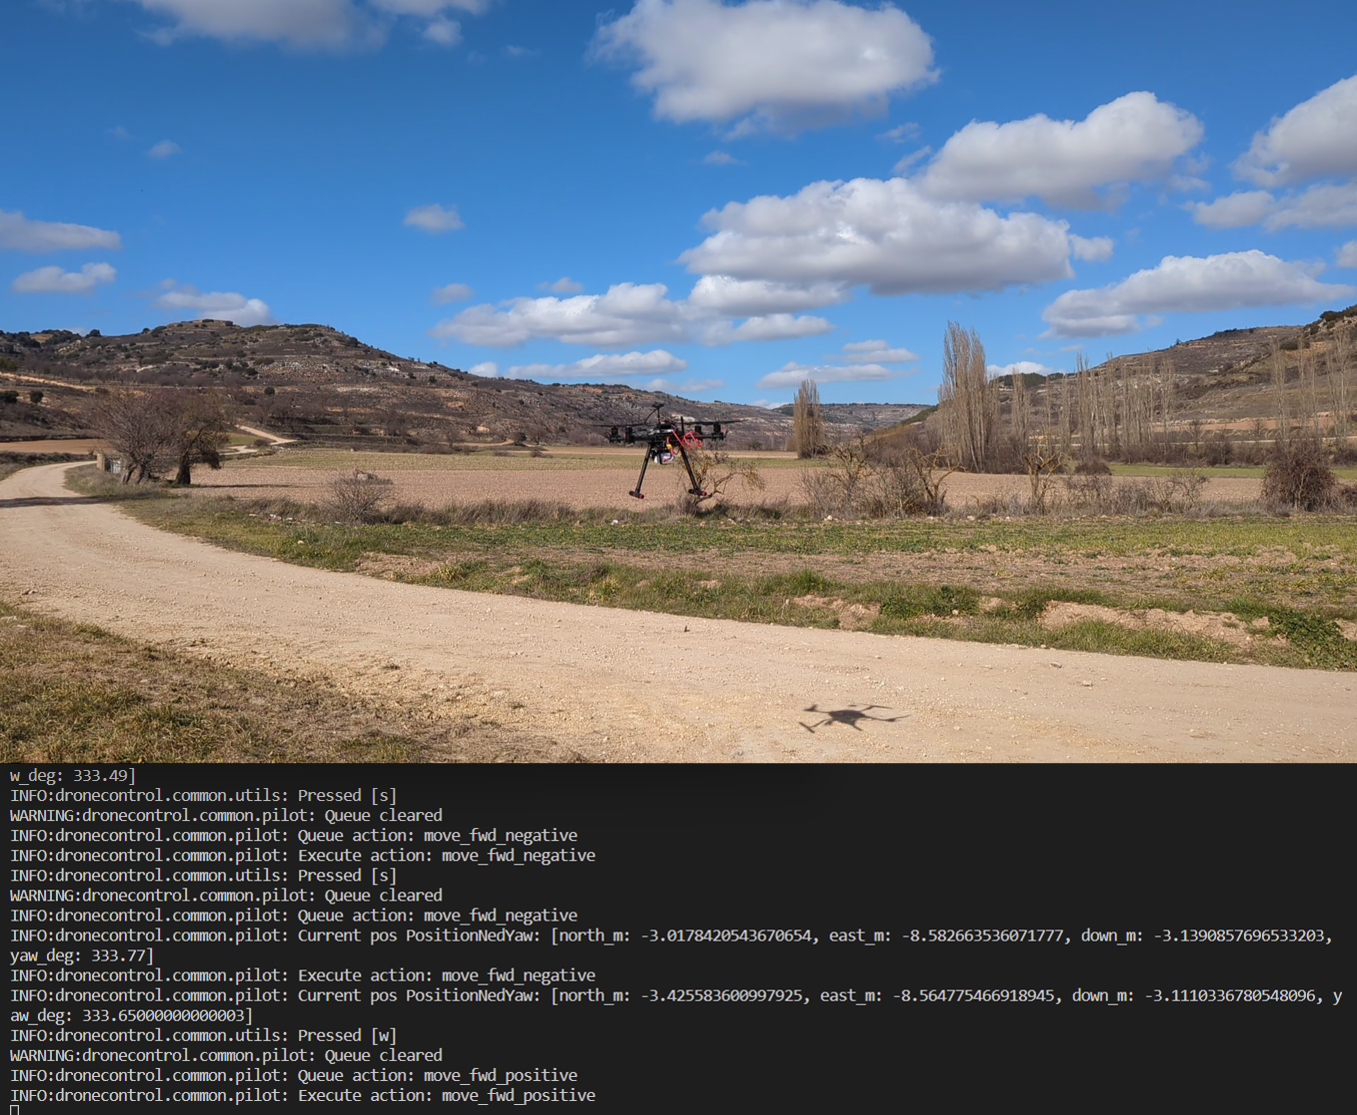
\includegraphics[width=\textwidth, keepaspectratio]{img/video-field-test-offboard.png}
  \caption{Terminal output from the \texttt{test-camera} tool running on an offboard computer and image of the drone flying in response}
  \label{fig:flight-test-cam-offboard}
\end{figure}

\subsubsection{Onboard computer flight with test tool}
\label{subsec:fl-test-3}

The third and last test flight in this section will ensure that the custom software can send takeoff and landing commands through a cabled MAVlink channel from the onboard computer,
as well as ensuring that the onboard camera can obtain a good image of the field of view of the vehicle during flight.
For that, the same tool will be used as in the last test, 
but in this instance, it will be run on the Raspberry Pi, and the connection will be established through the wired serial link between this onboard computer and the Pixhawk autopilot board.
Since the camera connected to the computer sending commands is now looking down on the pilot, it is possible to activate pose detection on the test images received from this onboard camera.
To start the flight test, the main and secondary batteries need to be attached, respectively, to the power module and to the Raspberry Pi.
After the onboard computer has started, the easiest way to control it is with a remote desktop connection through WiFi, as explained in section \ref{sec:devenv}.
By this connection, a terminal window can be opened on the desktop, and the following command run:
\begin{minted}[breaklines, fontsize=\footnotesize, baselinestretch=1]{bash}
dronecontrol tools test-camera -r /dev/serial0:921600 -p
\end{minted}
As opposed to the flight using the telemetry radio, in this test the serial connection runs at a baudrate of 921600, which matches the configured baudrate on the \texttt{TELEM2} port of the Pixhawk board.
The "-p" option enables pose detection in the output images.
A video of the entire process can be found \href{https://l-gonz.github.io/tfg-giaa-dronecontrol/videos/flight-test-onboard}{here}\footnote{\url{https://l-gonz.github.io/tfg-giaa-dronecontrol/videos/flight-test-onboard}} and an image extracted form it can be seen in figure \ref{fig:flight-test-cam-onboard}.


\begin{figure}
  \centering
  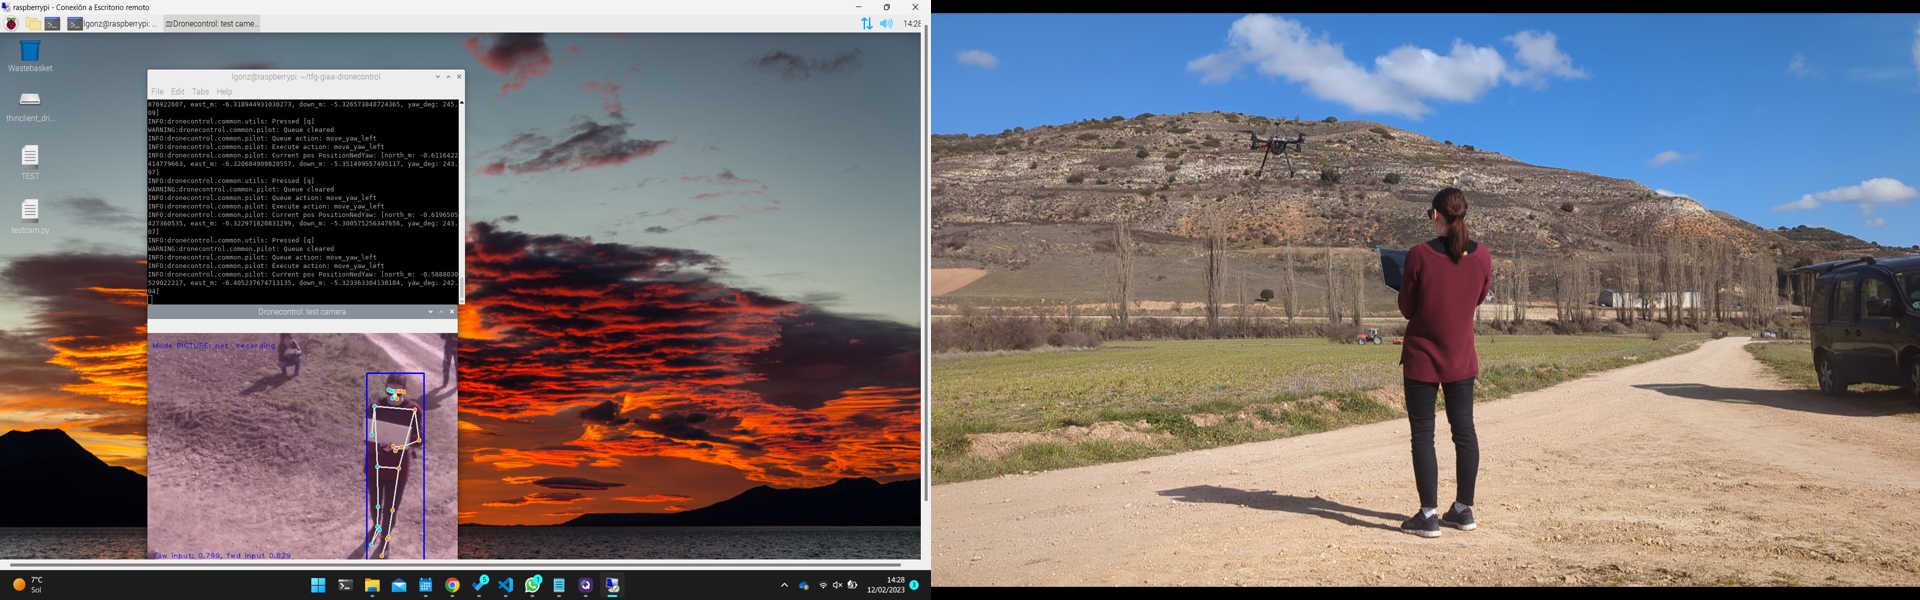
\includegraphics[width=\textwidth, keepaspectratio]{img/video-field-test-onboard.png}
  \caption{Pose detection algorithm running on images taken during flight}
  \label{fig:flight-test-cam-onboard}
\end{figure}


\subsection{Hand gesture control}
\label{subsec:fl-test-4}

% Setup:    ...
% Test:     - Hand solution on windows through telemetry radio
%           - Free movement with offboard api
% Results:  video of flying, output from program

During basic flight tests, all the connections and individual parts of the software were validated in actual flight.
Now, it is time to integrate the piloting system with the image recognition results to test the developed vision-based control solutions.
The first solution to be used in flight will be the hand-gesture guidance system, which runs on an offboard computer with more available processing resources and no dependence on battery-supplied power to work.
The setup will be identical to the second test flight (\ref{subsec:fl-test-2}) with the telemetry radio as the serial link and the onboard companion computer turned off
Once the autopilot board is powered up, the control solution can be started with the following command:
\begin{minted}[breaklines, fontsize=\footnotesize, baselinestretch=1]{bash}
dronecontrol hand -s <device>:57600
\end{minted}
where <device> is the COM port or TTY device the telemetry radio is attached to, depending on the platform.


After the pilot connects, the image from the computer's webcam will appear on the screen with an outline over any detected hand.
An open palm should be shown to the camera to start controlling the vehicle.
Then, a closed fist will make the drone take off, and pointing up with the index finger will start the offboard flight mode.
Afterwards, moving the index finger right or left will make the vehicle mirror the movement, 
and moving the thumb right or left will make the vehicle move forward and backwards, respectively.
At any point during the test, an open hand will make the drone hover at its current place, as will losing sight of the controlling hand.
A video of the entire process can be found \href{https://l-gonz.github.io/tfg-giaa-dronecontrol/videos/flight-test-hand}{here}\footnote{\url{https://l-gonz.github.io/tfg-giaa-dronecontrol/videos/flight-test-hand}} and an image extracted form it can be seen in figure \ref{fig:flight-test-hand}.

\begin{figure}
  \centering
  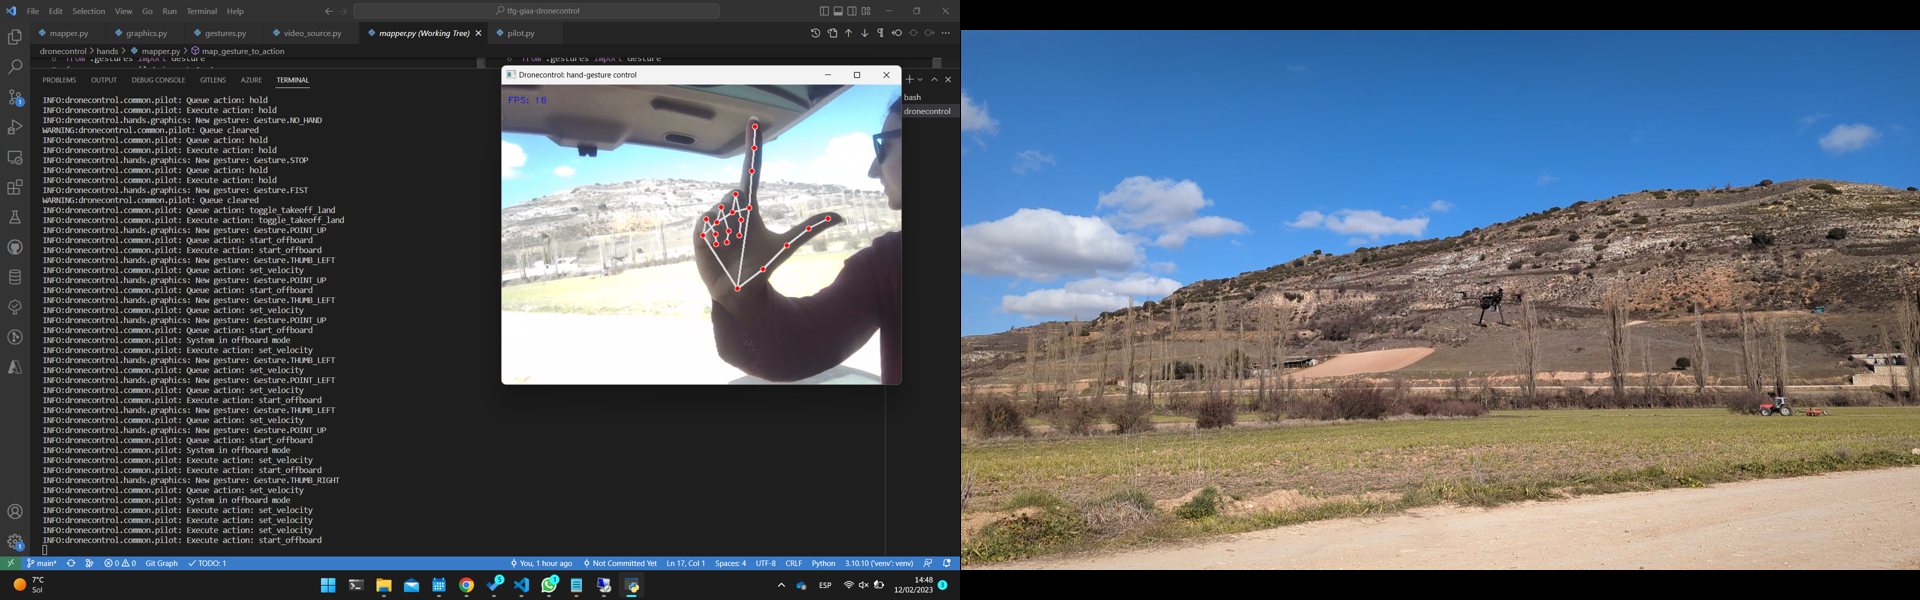
\includegraphics[width=\textwidth, keepaspectratio]{img/video-field-test-hand.png}
  \caption{Image taken during flight controlled by the hand-gesture solution. The vehicle is moving forward.}
  \label{fig:flight-test-hand}
\end{figure}

\subsection{Target detecting, tracking and following}
\label{subsec:fl-test-5}

% Setup:    ...
% Test:     - Follow solution on RPi
%           - Controller response to real input
% Results:  video of flying, output from program

Finally, it only remains to test the follow control solution.
In this section, the companion computer will be running the follow program, and it will be validated whether it can keep track of and follow a moving target during a non-simulated flight.
The setup will be identical to the third test in section \ref{subsec:fl-test-3}, without needing a wireless telemetry connection.
The telemetry radio is, therefore, free to be used, for example, to track the vehicle's path through the QGroundControl application on a secondary, offboard computer.
The control application will be started with the following command:
\begin{minted}[breaklines, fontsize=\footnotesize, baselinestretch=1]{bash}
dronecontrol follow -s /dev/serial0:921600
\end{minted}
This \href{https://l-gonz.github.io/tfg-giaa-dronecontrol/videos/flight-test-follow}{video}\footnote{\url{https://l-gonz.github.io/tfg-giaa-dronecontrol/videos/flight-test-follow}} shows the process of getting the vehicle to takeoff (T key), activating offboard flight mode (O key), and starting movement tracking of the detected figure.
Figure \ref{fig:flight-test-follow} shows an image extracted from this video.


\begin{figure}
  \centering
  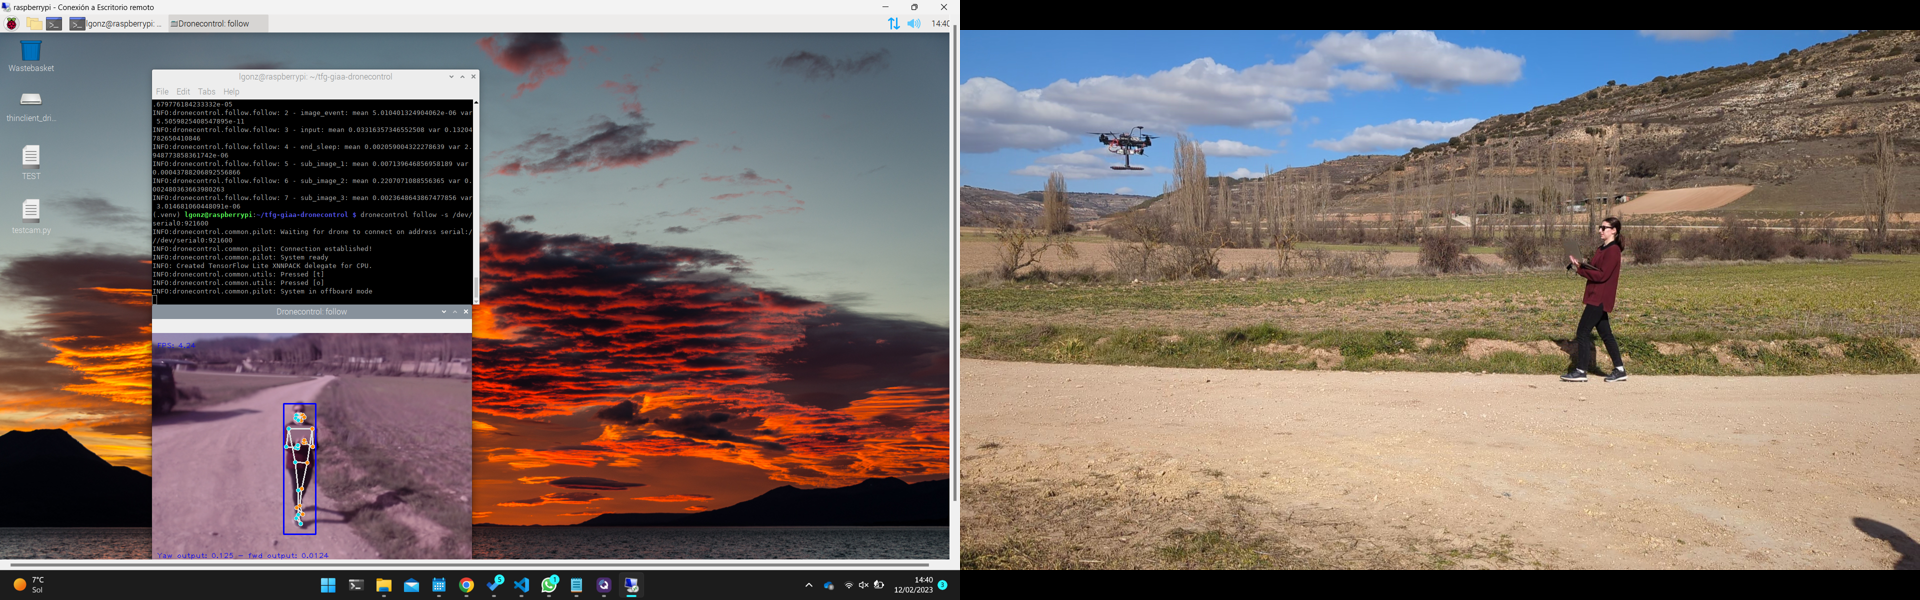
\includegraphics[width=\textwidth, keepaspectratio]{img/video-field-test-follow.png}
  \caption{Terminal and image output of the dronecontrol follow solution running on the Raspberry Pi}
  \label{fig:flight-test-follow}
\end{figure}

The maximum frames per second managed by the program running on the Pi is around 6 FPS when the follow mechanism is engaged and around 8 FPS if it is disabled by switching out of offboard flight mode.
In practice, this means that the person being tracked by the drone has to move quite slowly for the camera not to lose sight of them before the autopilot can send the command to the vehicle to move to the previously detected position.
However, for a proof-of-concept scenario, this is an acceptable performance.
At the end of the program run, the average loop time and average runtime for each of the tasks in the main loop are shown in the terminal.
From the measures obtained for the test flight carried out, the average frame rate calculates to be 3.58 FPS.
If these measurements are compared to those analyzed in section \ref{subsec:performance}, as shown in figure \ref{fig:flight-performance}, particularly to the test configuration most closely resembling actual flight with the autopilot board running on HITL mode and the companion computer powered by the secondary battery, it is possible to appreciate how close this configuration matches the behaviour during actual flight and therefore validating it as an appropriate environment to test the performance of this type of algorithms.


\begin{figure}
  \centering
  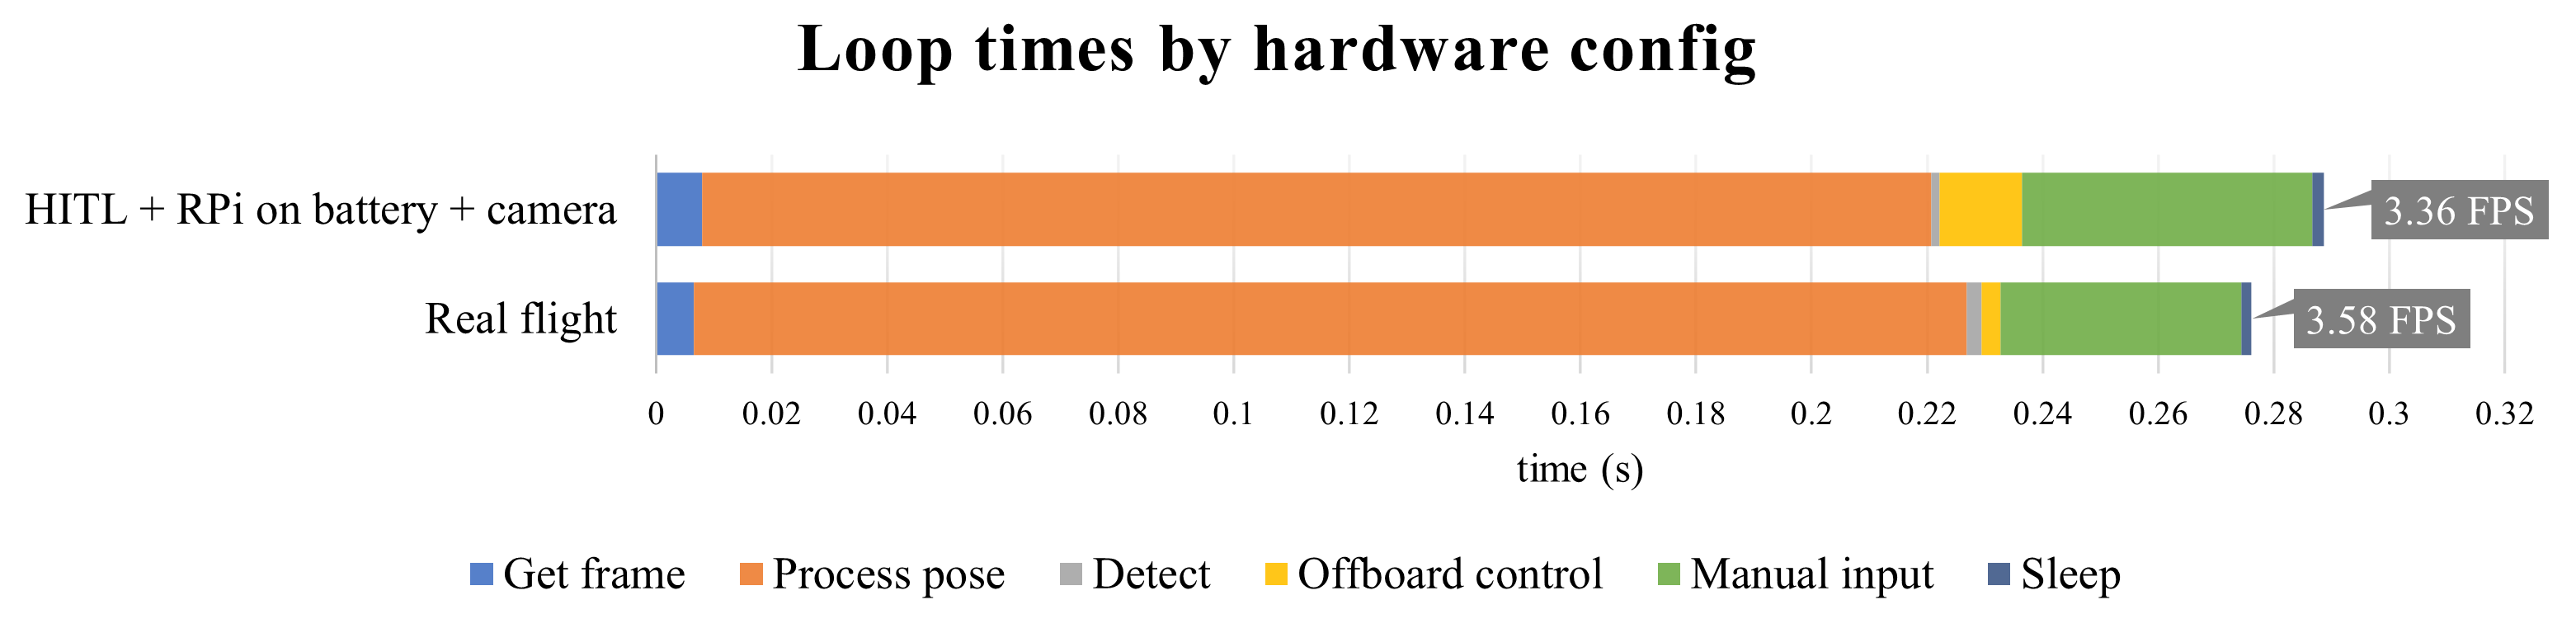
\includegraphics[width=0.9\textwidth, keepaspectratio]{img/perf-hitl-flight.png}
  \caption{Terminal and image output of the dronecontrol follow solution running on the Raspberry Pi}
  \label{fig:flight-performance}
\end{figure}
